\documentclass{cmc}
\usepackage{makecell}

\begin{document}

\pagestyle{fancy}
\lhead{\textit{\textbf{Computational Motor Control, Spring 2020} \\
    Final project, Lab 8, GRADED}} \rhead{Genilloud, Fernandez, Dunant}

\subsection*{Student names: Genilloud Florian, Emilio Fernandez, Joachim Dunant}

\section*{Swimming with Salamandra robotica – CPG Model}
\label{sec:exploring-swimming}

In this project you will control a salamander-like robot Salamandra
robotica II for which you will use Python and the PyBullet physics
engine. Now you have an opportunity to use what you’ve learned until
now to make the robot swim and eventually walk. In order to do this,
you should implement a CPG based swimming controller, similarly to the
architecture shown in Figure~\ref{fig:controller-model}.

The project is based on the research of \cite{Crespi2013},
\cite{Karakasiliotis2013} and \cite{ijspeert2007swimming}. It is strongly
recommended to review \cite{ijspeert2007swimming} and its supplementary material
provided on the Moodle. You will be tasked with replicating and
studying the Central Pattern Generator (CPG).

\begin{figure}[h]
  \centering
  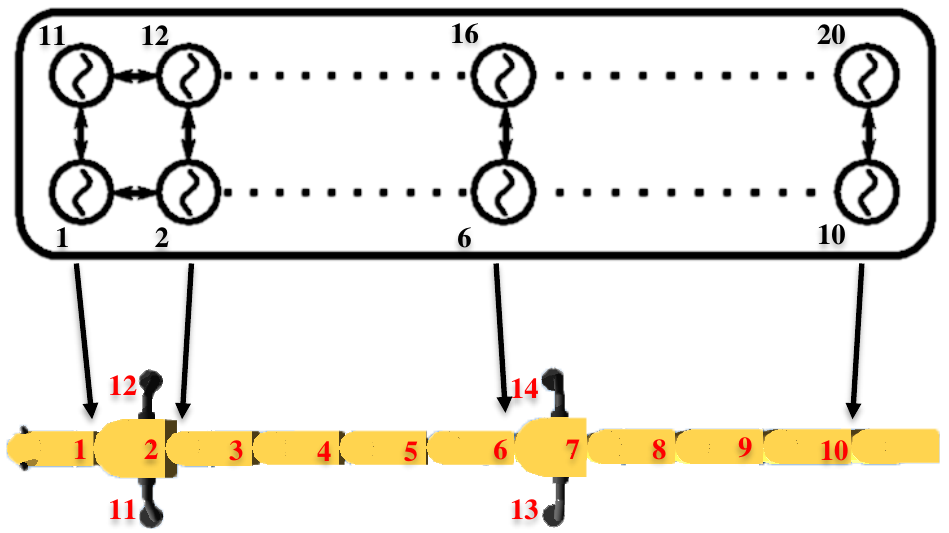
\includegraphics[width=0.5\textwidth]{figures/model_controller.png}
  \caption[Controller model]{A double chain of oscillators controlling
    the robot’s spine.}
  \label{fig:controller-model}
\end{figure}

\textbf{Fun fact:} The salamander's name is T-Rex V.3141592

\subsection*{8a. Implement a double chain of oscillators along with
  limb CPG's}
\label{sec:implement-chain}

Salamandra robotica has 10 joints along its spine and 1 joint for each
limb. The controller is defined as

\begin{equation}
  \label{eq:dphase}
  \dot{\theta}_i = 2 \pi f + \sum_j r_j w_{ij} sin(\theta_j - \theta_i - \phi_{ij})
\end{equation}

\begin{equation}
  \label{eq:dr}
  \dot{r}_i = a (R_i - r_i)
\end{equation}

\begin{equation}
  \label{eq:output}
  q_i = r_i(1 + cos(\theta_i)) - r_{i+10}(1 + cos(\theta_{i+10})) \text{ if body joint}
\end{equation}

with $ \theta_i $ the oscillator phase, f the frequency, $ w_{ij} $ the coupling
weights, $ \phi_{ij} $ the nominal phase lag (phase bias), $ r_i $ the
oscillator amplitude, $ R_i $ the nominal amplitude, $ a $ the convergence
factor and $ q_i $ the spinal joint angles. For more information, please refer
to \cite{ijspeert2007swimming}. Also note how these are the same equations,
although Equation \eqref{eq:dr} has been simplified into a first order ODE in
order to simplify the implementation in this project.


\begin{enumerate}
\item We have implemented the double chain oscillator model by including equations \ref{eq:dphase} and \ref{eq:dr} in the function \fileref{network.py::network\_ode}. The parameters appearing in those equations are defined in \fileref{robot\_parameters.py} and in \fileref{simulation\_parameters.pys} using the following information obtained from the supporting material for \cite{ijspeert2007swimming}:


\begin{figure}[h!]
    \centering
        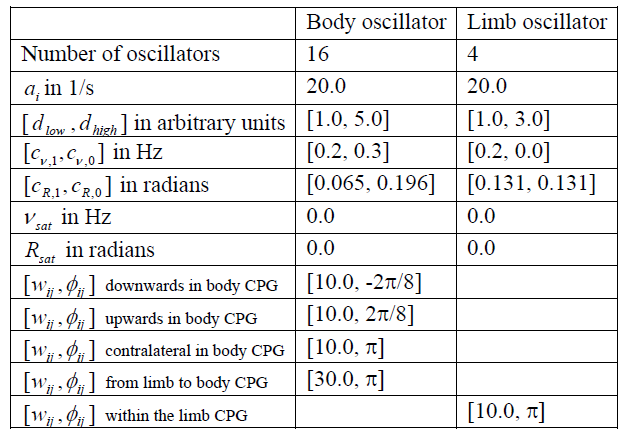
\includegraphics[width=0.6\textwidth]{figures/parameters.PNG} 
    \caption{Parameters for CPG model} 
    \label{fig:parameters}                            
\end{figure}

\newpage

\begin{figure}[h!]
    \centering
        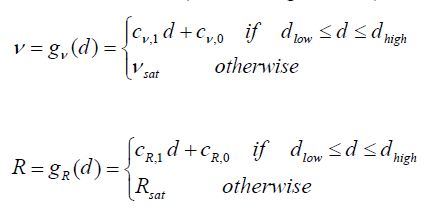
\includegraphics[width=0.45\textwidth]{figures/saturation_function.PNG} 
    \caption{Saturation functions for frequencies and nominal amplitudes}
    \label{fig:saturation}                            
\end{figure}

The weights and phase bias are set with a 24x24 matrix after reading a csv file defined as described in \ref{fig:parameters}. The rest of the parameters are used for defining the saturation functions in \ref{fig:saturation}.
Finally, we test out implementation by running the network using \fileref{run\_network.py}.

\item We implement the output of your CPG network in the function
  \fileref{network.py::motor\_output} to generate the body spinal joint
  angles according to equation \ref{eq:output}. For the phase spinal joints we simply take the value of the phase if the amplitude is non-zero

\item Finally, we implement an increasing drive in order to show that our network can generate swimming and walking patterns similarly to \cite{ijspeert2007swimming}. We will know compare our resulting plots with the  "model" plots in \ref{fig:science_oscillator_patterns} and \ref{fig:science_oscillator_properties} obtained from \cite{ijspeert2007swimming}
\end{enumerate}


\begin{figure}[h]
  \centering
  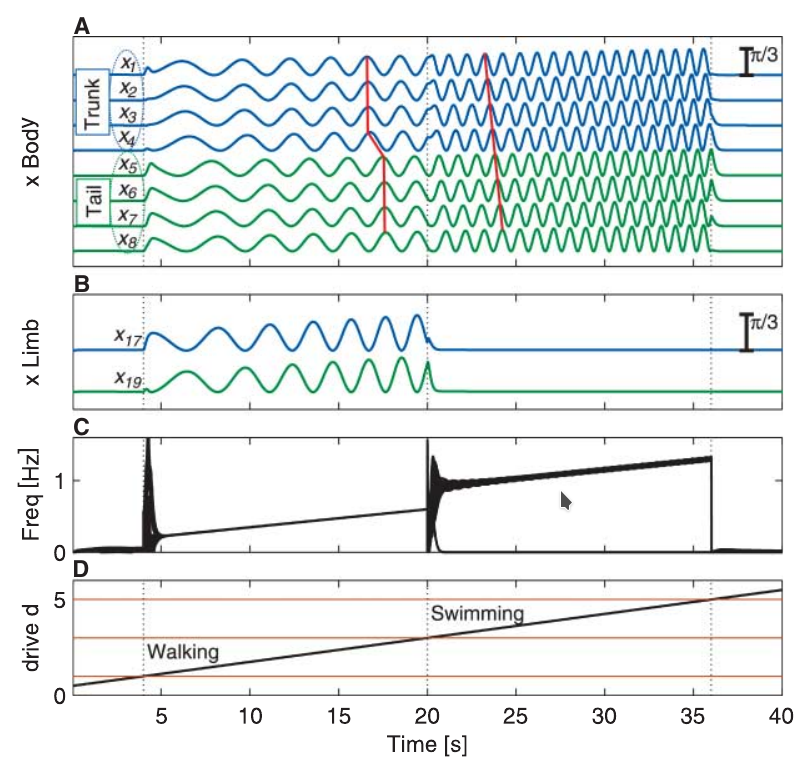
\includegraphics[width=0.55\textwidth]{figures/science_oscillator_patterns}
  \caption{Oscillator patterns from \cite{ijspeert2007swimming}}
  \label{fig:science_oscillator_patterns}
\end{figure}


\begin{figure}[H] 
  \begin{subfigure}[b]{0.5\linewidth}
    \centering
    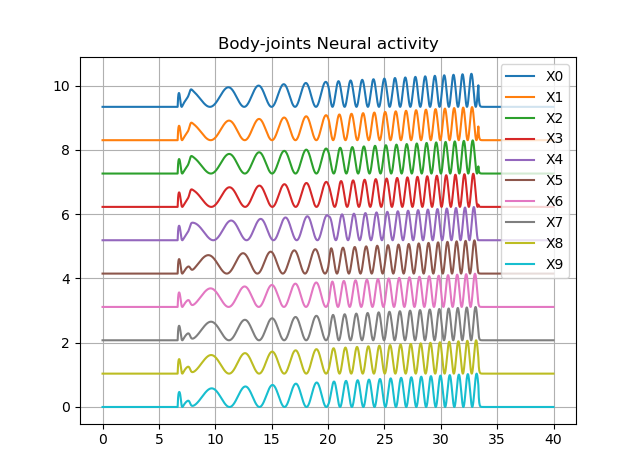
\includegraphics[width=1\linewidth]{figures/Figure_3.png} 
    \caption{Body joints output} 
    \label{fig:oscillation:a} 
  \end{subfigure}%% 
  \begin{subfigure}[b]{0.5\linewidth}
    \centering
    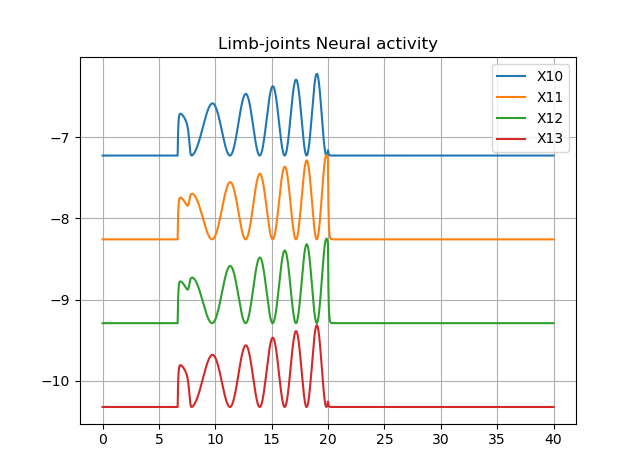
\includegraphics[width=1\linewidth]{figures/Figure_4.png} 
    \caption{Limb joints output} 
    \label{fig:oscillation:b} 
  \end{subfigure} 
  \begin{subfigure}[b]{0.5\linewidth}
    \centering
    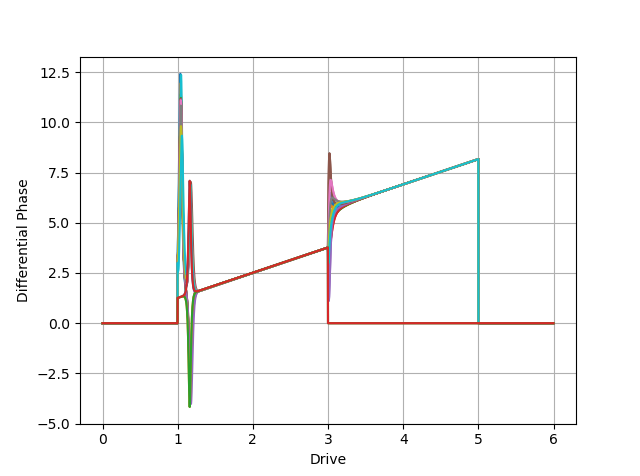
\includegraphics[width=1\linewidth]{figures/Differential_phase.png} 
    \caption{Frequency} 
    \label{fig:oscillation:c} 
  \end{subfigure}%%
  \begin{subfigure}[b]{0.45\linewidth}
    \centering
    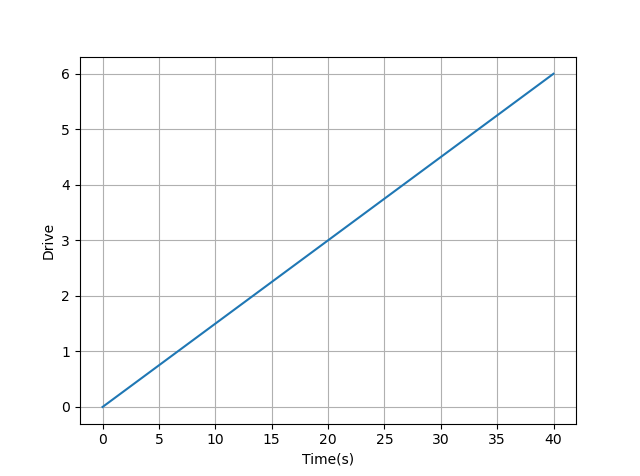
\includegraphics[width=1\linewidth]{figures/Drive.png} 
    \caption{Drive} 
    \label{fig:oscillation:d} 
  \end{subfigure} 
  \caption{Oscillation patterns from our network (compare with Fig. \ref{fig:science_oscillator_patterns})}
  \label{fig:oscillation} 
\end{figure}

\textbf{Oscillation patterns comparison:} Above we have the oscillation patterns generated from our network. First of all, we observe that the drive (Figure \ref{fig:oscillation:d} is identical to the one shown in \ref{fig:science_oscillator_patterns}.D: it increases from 0 to 6 during 40 seconds, so that the salamander can walk (after 4 secs) and swim (after 20 secs). Figure \ref{fig:oscillation:a} and \ref{fig:oscillation:b} are obtained using the equation $q_i = r_i(1 + cos(\theta_i))$, which corresponds to the output neural activities for all the activities. They behave as expected: during walking we observe a standing wave with long cycle duration, whereas during swimming we observe a shorter-cycle duration travelling wave in body joints and the limb joints are tonic. Finally, Figure \ref{fig:oscillation:c} shows the differential phases (in radians). If we compare it with the "model" plot (\ref{fig:science_oscillator_patterns}.C we observe that they have a similar shape: there's a burst when the salamander starts walking as well as when the salamander starts swimming. Probably the first burst could be improved in our network, there might be a problem with the motor outputs at the beginning of the simulation. In general, we can conclude that we have successfully reproduced the oscillation patterns from \cite{ijspeert2007swimming}.


\textbf{Oscillation properties comparison:} We have already verify the correct functioning of our network. Nonetheless, we also want to compare the oscillation properties of our network, especially the saturation functions shown in Figure \ref{fig:saturation_plot}. We observe that their behavior is identical to Figure \ref{fig:science_oscillator_properties}(A and B). The body joints are "active" during both walking and swimming whereas the limb joints are only active during walking because they saturate during swimming. We also see that limb joints oscillate with lower frequency but with higher amplitude than body joints.

\begin{figure}[h]
  \centering
  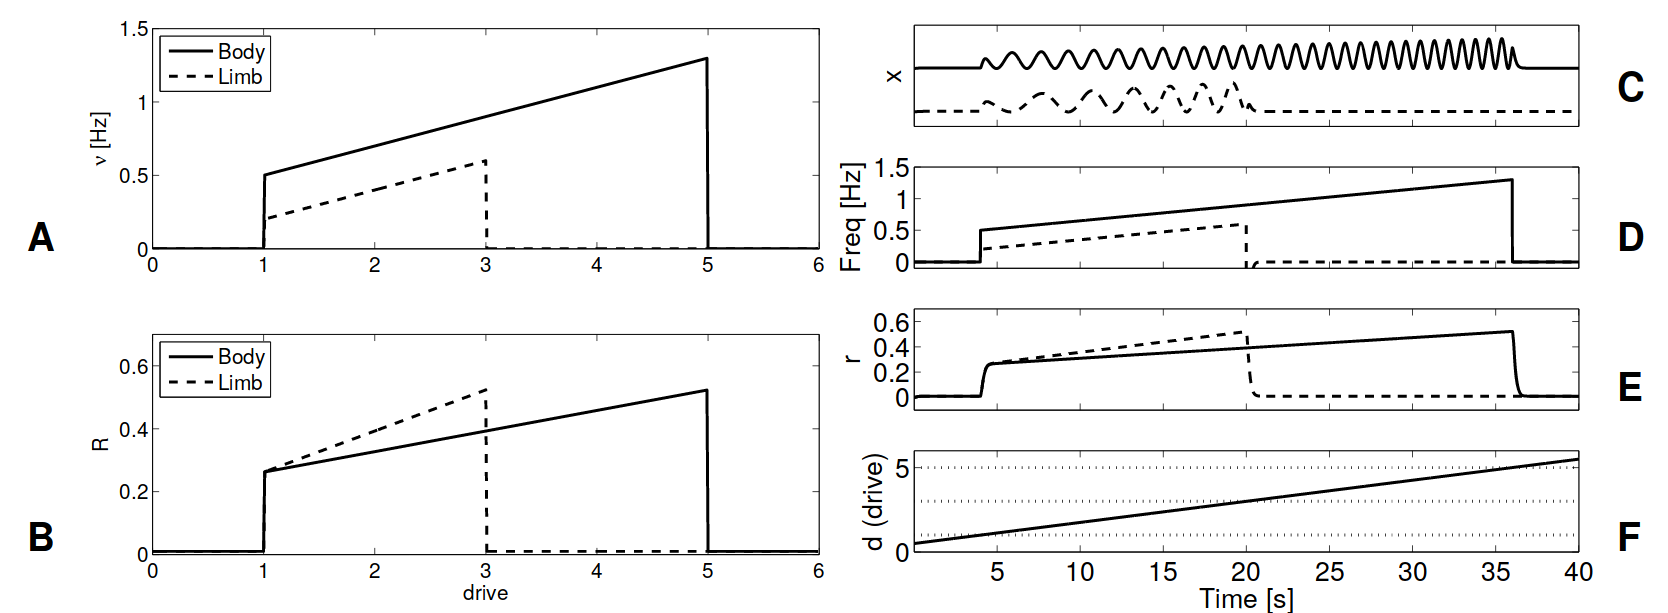
\includegraphics[width=0.8\textwidth]{figures/science_oscillator_properties}
  \caption{Oscillator properties from \cite{ijspeert2007swimming} supplementary material}
  \label{fig:science_oscillator_properties}
\end{figure}

\begin{figure}[H] 
  \begin{subfigure}[b]{0.5\linewidth}
    \centering
    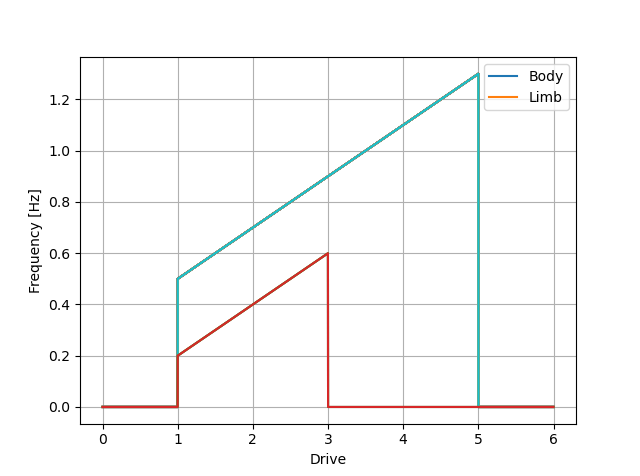
\includegraphics[width=0.75\linewidth]{figures/Frequency_for_joints.png} 
    \caption{Frequency} 
    \label{fig:saturation_plot:a} 
  \end{subfigure}%% 
  \begin{subfigure}[b]{0.5\linewidth}
    \centering
    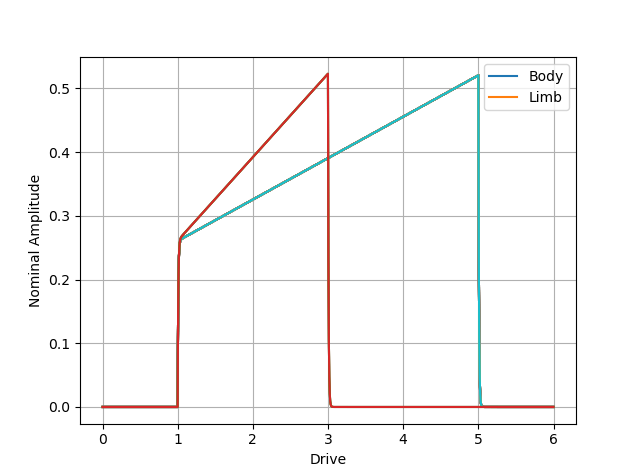
\includegraphics[width=0.75\linewidth]{figures/Amplitude_for_joints.png} 
    \caption{Nominal amplitude} 
    \label{fig:saturation_plot:b} 
  \end{subfigure} 
  \caption{Saturation functions from our network (compare with Fig \ref{fig:science_oscillator_properties})}
  \label{fig:saturation_plot} 
\end{figure}


\subsection*{8b. Effects of amplitude and phase lags on swimming
  performance}
\label{sec:amplitude-phase-performance}
 In this exercise, we study how does phase lag and oscillation amplitude influence the speed and energy.  We run a grid search in file \corr{exercise\_8b.py}
to explore the robot behavior for different combinations of amplitudes and phase
lags. The drive is set to 4 so that the salamander can swim and the frequency is set to 1 Hz. The amplitude will vary from 0.1 to 0.9 in and the phase lag will vary from 0 to $\pi$ rads. In total, we use 100 samples (10 different amplitudes and 10 different phase lags). We tried to speed up the simulation by setting \texttt{fast} and \texttt{headless} to \textit{True}, and it took around 16 minutes to do the simulation (10 secs per simulation).

\begin{figure}[H] 
  \begin{subfigure}[b]{0.5\linewidth}
    \centering
    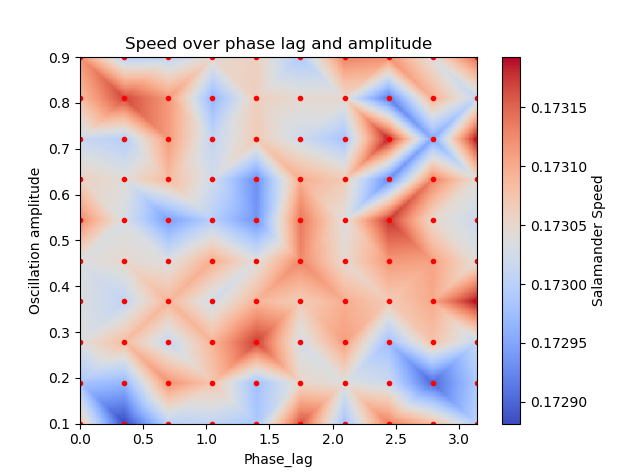
\includegraphics[width=0.9\linewidth]{figures/Speed.png} 
    \caption{Speed (m/s)} 
    \label{fig:exercise8b_results:a} 
  \end{subfigure}%% 
  \begin{subfigure}[b]{0.5\linewidth}
    \centering
    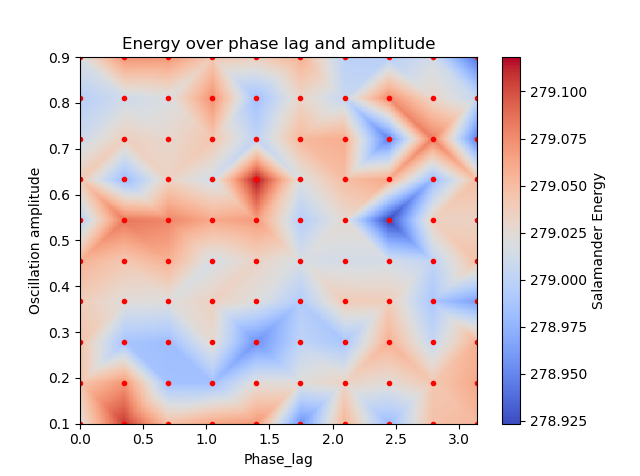
\includegraphics[width=0.9\linewidth]{figures/Energy.png} 
    \caption{Energy (J)} 
    \label{fig:exercise8a_results:b} 
  \end{subfigure}
  \caption{Grid search results}
  \label{fig:exercise8b_results} 
\end{figure}


 We use the function \corr{plot\_results.py::exercise8b\_gridsearch()} to load and plot the logged data from the simulation including 2D/3D plots showing our grid search results. The metrics we are interested in are speed and energy. Speed is computed by adding the mean speed of the salamander head along the x-coordinate and the y-coordinate. Energy  is computed by integrating the product of the joint torques and velocities. The grid search results for both metrics are shown in Figure \ref{fig:exercise8b_results}. At the end, our aim is to obtain the best combination of amplitude and phase lag which yields the highest speed and the lowest energy. For that purpose, we create another metric called \textit{performance} which is simply the speed divided by the energy. In Figure \ref{fig:exercise8b_performance}, we observe that the best performance occurs for amplitude=0.55 and phase\_lag=2.5 rads.

\begin{figure}[H]
  \centering
  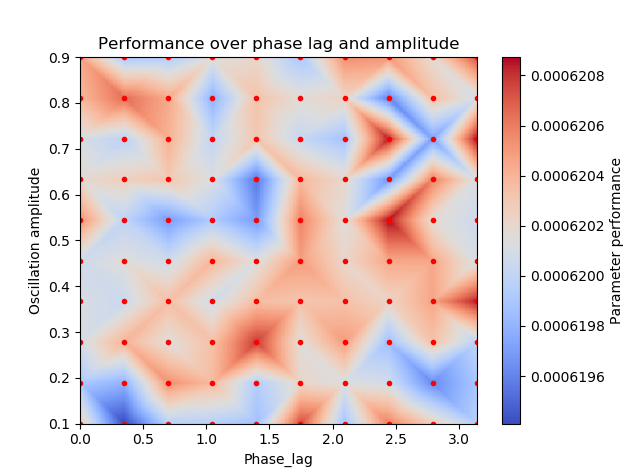
\includegraphics[width=0.7\textwidth]{figures/Performance.png}
  \caption{Grid search results for performance}
  \label{fig:exercise8b_performance}
\end{figure}

Once we have found the best combination, we plot the salamander trajectory and positions for the simulation corresponding to the most performing combination of amplitude and phase lag, using the function  \corr{plot\_results.py :: plot\_efficient\_behaviour(i)}. The resulting plots are shown in Figure \ref{fig:exercise8b_behaviour} and we observe that, although the salamander is moving forward, there is room for improvement because it is oscillating too much. This issue will be solved in the following exercises.

\begin{figure}[H] 
  \begin{subfigure}[b]{0.5\linewidth}
    \centering
    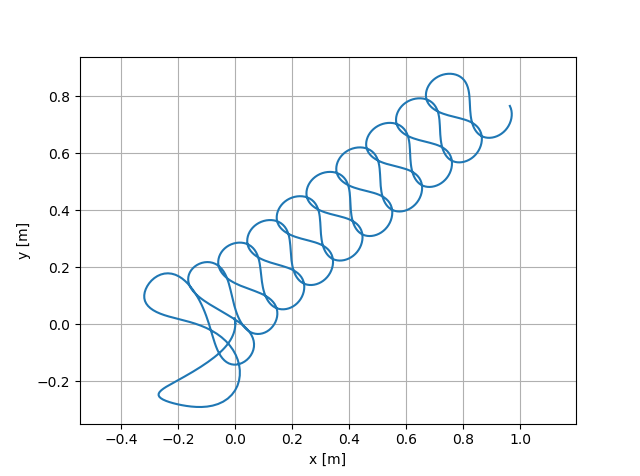
\includegraphics[width=0.9\linewidth]{figures/Trajectory.png} 
    \caption{Trajectory} 
    \label{fig:exercise8b_behaviour:a} 
  \end{subfigure}%% 
  \begin{subfigure}[b]{0.5\linewidth}
    \centering
    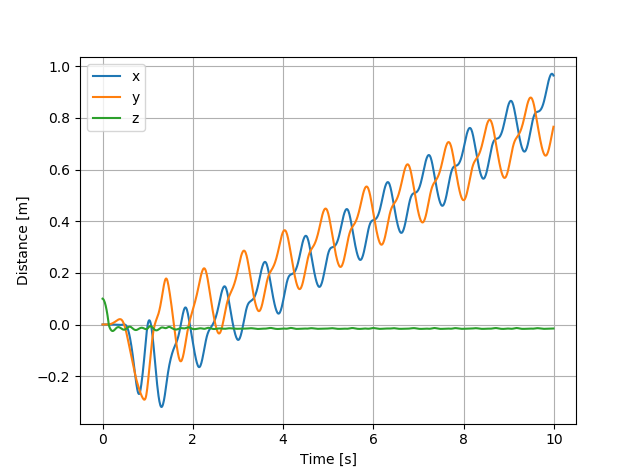
\includegraphics[width=0.9\linewidth]{figures/Positions.png} 
    \caption{Positions} 
    \label{fig:exercise8a_behaviour:b} 
  \end{subfigure}
  \caption{Salamander behaviour for lowest energy and highest speed}
  \label{fig:exercise8b_behaviour} 
\end{figure}




\subsection*{8c. Amplitude gradient}
\label{sec:amplitude-gradient}
In this exercise, we study how does an amplitude's gradient influence the speed and the energy of the salamander. Therefore we used two parameters: amplitudes of the first (Rhead) and last
  (Rtail) oscillator in the spine (corresponding to the first and last
  motor). To do so, you can add a parameter amplitudes=[Rhead, Rtail] in
  \corr{simulation\_parameters.py::SimulationParameters}. The goal of this step is to have a smooth movements in the salamander. When we have the parameters (Rhead) and (Rtail), we just have to compute the gradient by using the numpy function linspace like :
 \begin{lstlisting}
    np.linspace(Rhead, Rtail,nb_body_joint)
 \end{lstlisting}
 Then, we use the function \corr{plot\_results.py::exercise\_8c\_plot\_gridsearch()} to load and plot the logged data from the simulation including 2D/3D plots showing our grid search results. We're interested by the metrics speed and energy. Those two metrics are computed exactly as in Section 8b. The amplitude gradient will vary from 0.3 to 1 for Rhead and Rtail which gives use 100 samples. As before, we tried to speed up the simulation and it took around 16 minutes to compute all the simulations (10 secondes per simulation).
 \begin{figure}[H] 
  \begin{subfigure}[b]{0.5\linewidth}
    \centering
    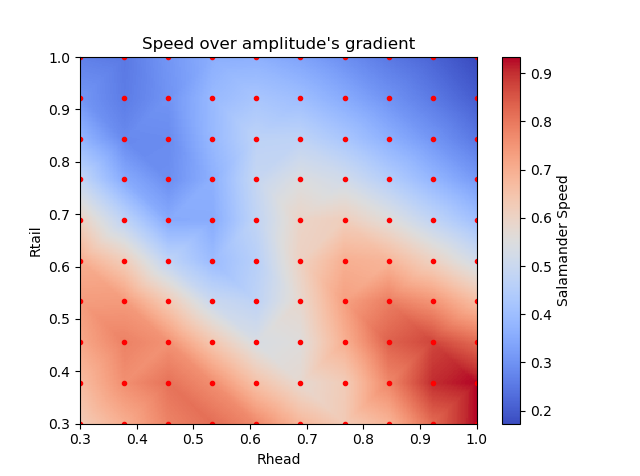
\includegraphics[width=0.9\linewidth]{figures/Speed_8c.png} 
    \caption{Speed (m/s)} 
    \label{fig:exercise8c_results:a} 
  \end{subfigure}%% 
  \begin{subfigure}[b]{0.5\linewidth}
    \centering
    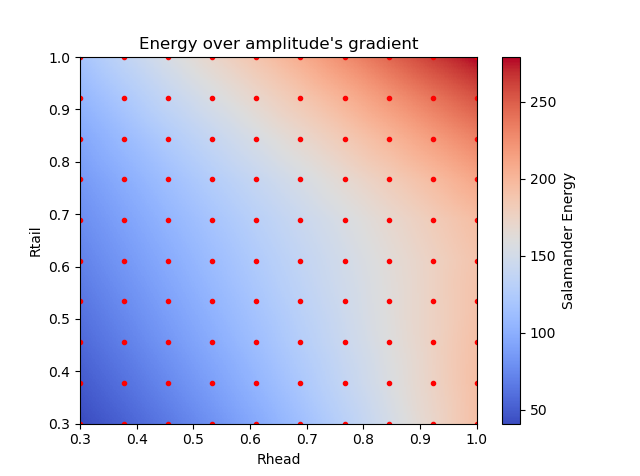
\includegraphics[width=0.9\linewidth]{figures/Energy_8c.png} 
    \caption{Energy (J)} 
    \label{fig:exercise8c_results:b} 
  \end{subfigure}
  \caption{Grid search results}
  \label{fig:exercise8c_results} 
\end{figure}

As we can see in Figure \ref{fig:exercise8c_results}, the speed and the energy of the robot varies as a function of the gradient of the amplitude. First, with the Figure \ref{fig:exercise8c_results:a}, we observe that if the amplitude of the head is higher that the amplitude of the tail, the robot will swim faster. Second, with Figure \ref{fig:exercise8c_results:b}, if the amplitude is set to the maximum for the head and the tail, the energy will be maximal which corresponds to the definition of the energy ( the more you have strength the more the energy will becomes). 

\begin{figure}[H]
  \centering
  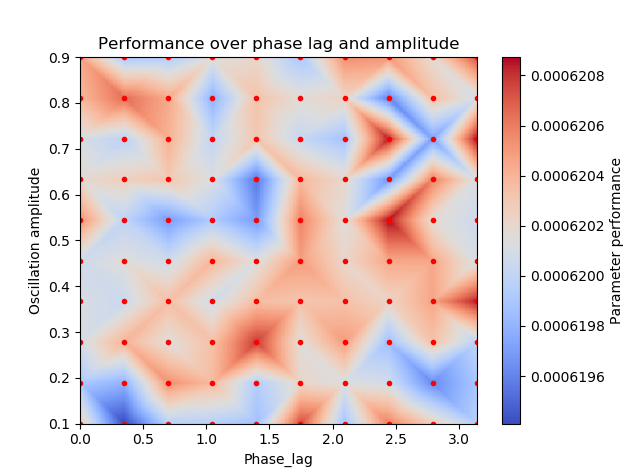
\includegraphics[width=0.7\textwidth]{figures/Performance.png}
  \caption{Phase lags along the spine during walking}
  \label{fig:exercise8c_phaseLag}
\end{figure}

Finally, as for section 8b, we compute the performance to find the best parameters and as shown in figure \ref{fig:exercise8c_results}, the best parameters are Rhead= 0.3 and Rtail = 0.3.
In comparison with the \corr{exercise\_8b.py}, the salamander move in a more straight forward direction as shown in the figures below:
\begin{figure}[H] 
  \begin{subfigure}[b]{0.5\linewidth}
    \centering
    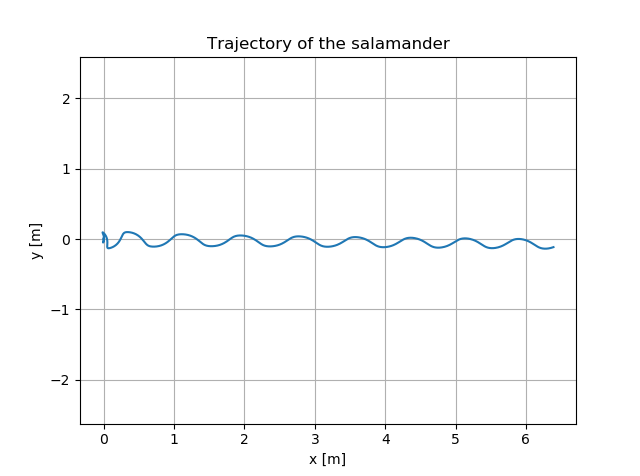
\includegraphics[width=0.9\linewidth]{figures/Trajectory_8c.png} 
    \caption{Trajectory} 
    \label{fig:exercise8c_behaviour:a} 
  \end{subfigure}%% 
  \begin{subfigure}[b]{0.5\linewidth}
    \centering
    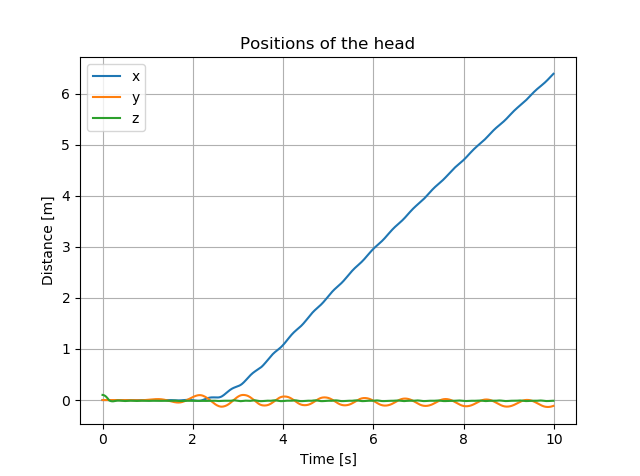
\includegraphics[width=0.9\linewidth]{figures/Positions_8c.png} 
    \caption{Positions} 
    \label{fig:exercise8c_behaviour:b} 
  \end{subfigure}
  \caption{Salamander behaviour for lowest energy and highest speed}
  \label{fig:exercise8c_behaviour} 
\end{figure}

 As we can see in figure \ref{fig:exercise8c_behaviour:b} where the movement along the x-axis is linear, meaning that its speed is constant. It shows that the body deformation is constant because of the phase lag being constant through the whole robot.

\subsection*{8d. Turning and backwards swimming}
\label{sec:turning-backwards}
For inducing turning, we can modulate the CPG network by decrease the nominal amplitude of one part of the body. In other words, if we decrease the nominal amplitude of the front part of the body, the salamander will turn left and if we decrease the nominal amplitude of the tail, the salamander will turn right.
The figures \ref{fig:exercise8d1_behaviour} below show the GPS trajectory and the spine angles while turning.
\begin{figure}[H] 
  \begin{subfigure}[b]{0.5\linewidth}
    \centering
    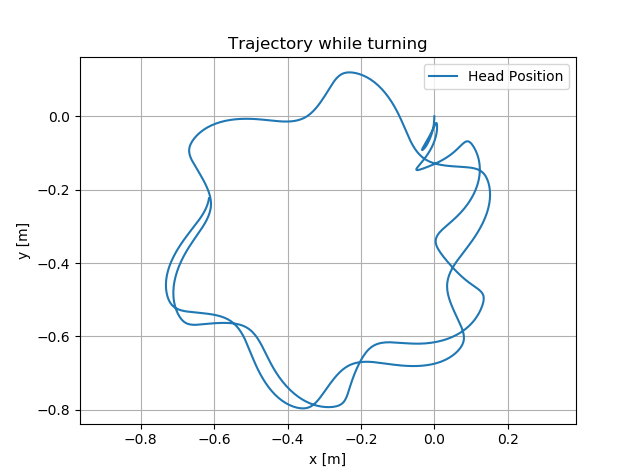
\includegraphics[width=0.9\linewidth]{figures/Trajectory_8d1.png} 
    \caption{Trajectory} 
    \label{fig:exercise8d1_behaviour:a} 
  \end{subfigure}%% 
  \begin{subfigure}[b]{0.5\linewidth}
    \centering
    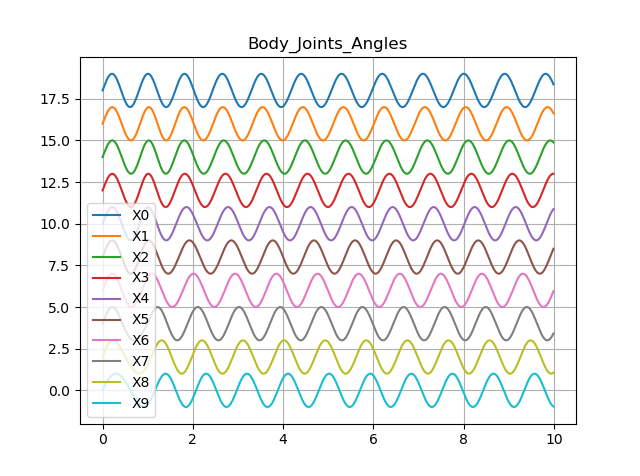
\includegraphics[width=0.9\linewidth]{figures/phase_angle_body_8d1.png} 
    \caption{Spine angles} 
    \label{fig:exercise8d1_behaviour:b} 
  \end{subfigure}
  \caption{Salamander trajectory and spine angles while turning}
  \label{fig:exercise8d1_behaviour} 
\end{figure}



Now, if we want to let the robot swim backwards, we just have to multiply each phase bias by $-1$. If we do so, the tail behaviour looks like the head and vice-versa.
The figures \ref{fig:exercise8d2_behaviour} below show the GPS trajectory and the spine angles while moving backwards.
\begin{figure}[H] 
  \begin{subfigure}[b]{0.5\linewidth}
    \centering
    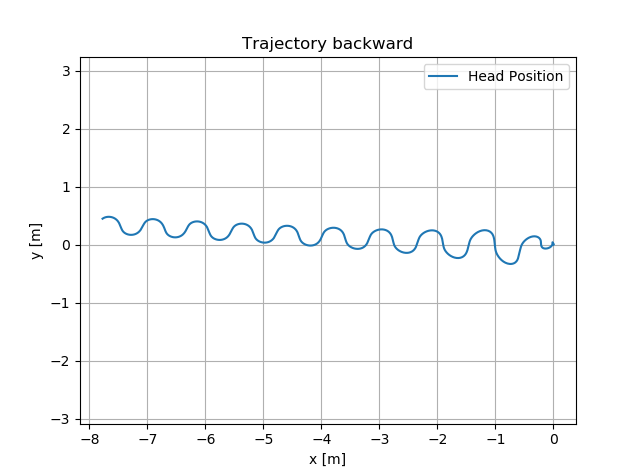
\includegraphics[width=0.9\linewidth]{figures/Trajectory_8d2.png} 
    \caption{Trajectory} 
    \label{fig:exercise8d2_behaviour:a} 
  \end{subfigure}%% 
  \begin{subfigure}[b]{0.5\linewidth}
    \centering
    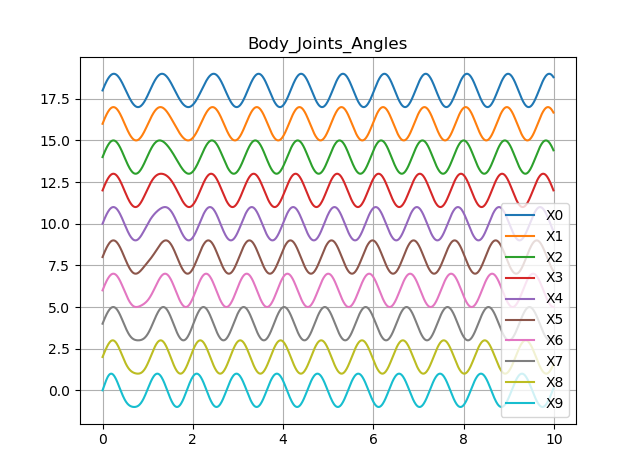
\includegraphics[width=0.9\linewidth]{figures/phase_angle_body_8d2.png} 
    \caption{Spine angles} 
    \label{fig:exercise8d2_behaviour:b} 
  \end{subfigure}
  \caption{Salamander trajectory and spine angles while turning}
  \label{fig:exercise8d2_behaviour} 
\end{figure}

It's interesting to see that if we let the robot swim backwards, the phase lag comes from the tail to the head.

\subsection*{8f. Limb – Spine coordination}
\label{sec:limb-spine-coordination}

In this part we explore the importance of a proper coordination between the spine and the limb movement for walking which is shown by the walking speed of the salamander. We do a parameter search over the nominal radius and phase offset between limb and body parts in \corr{exercise\_8f.py} to find what are the most optimal values.

Firstly, by changing only the drive to have a walking movement we find that indeed the graph of phase lags along the spine over time looks exactly like a walking movement where the upper part of the body has a single phase lag with the lower part, compared to swimming one which has a constant offset through the whole body.

\begin{figure}[H]
  \centering
  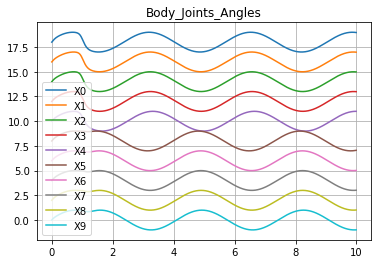
\includegraphics[width=0.7\textwidth]{figures/8f_phaseLagsBody.png}
  \caption{joint angles along the spine, showing the phase lags through the whole body}
  \label{fig:8f_phaseLagsBody}
\end{figure}

Then we lock the nominal radius to $0.3$ and change the phase offset from $0.1$ to $1.0$ and plot the speed of the head along the x-axis to compute the optimal value and once computes we do the opposite : Lock the phase offset as the previous found optimal value and do a parameter search over the nominal radius.

\begin{figure}[H] 
  \begin{subfigure}[b]{0.5\linewidth}
    \centering
    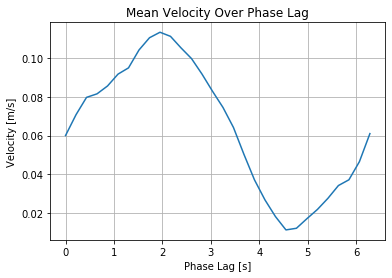
\includegraphics[width=0.9\linewidth]{figures/8f1_velocity_over_phase.png} 
    \caption{Speed over phase offset with nominal radius = 0.3[m]} 
    \label{fig:exercise8f1_results:a} 
  \end{subfigure}%% 
  \begin{subfigure}[b]{0.5\linewidth}
    \centering
    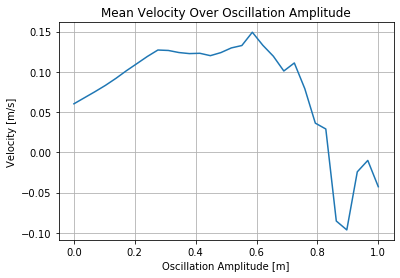
\includegraphics[width=0.9\linewidth]{figures/8f2_velocity_over_oscillation.png} 
    \caption{Speed over oscillation with phase offset = 1.95[s]} 
    \label{fig:exercise8f2_results:b} 
  \end{subfigure}
  \caption{Velocity over phase offset and oscillation amplitude}
  \label{fig:exercise8f_results} 
\end{figure}

We can see from the first graph that it has a sinusoidal shape with the highest being at $1.9499540608488373$. This plot shows that a lower value is more optimal, which could be explained by how the body moves while walking : The upper and low part of the body undulating in an opposite, symmetrical way. So, if the offset is too big then it will take more time to have a push from the limbs thus be slower overall.

Then the second plot shows that it is pretty constant until around $2\pi$ where it drops suddenly, because the body will turn too much over itself as shown in Figure \ref{fig:8f_oscillation}. Otherwise the velocity slowly increases until $0.5862068965517241$, the maximum value. This shows that a greater amplitude is better until it is not realistic anymore, because the limbs are able to push the body in a more efficient way.

\begin{figure}[H]
  \centering
  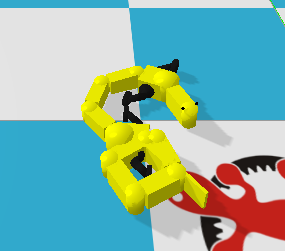
\includegraphics[width=0.7\textwidth]{figures/8f_oscillation_0_9.png}
  \caption{Problem occurring if the oscillation amplitude is too big (here 0.9[m])}
  \label{fig:8f_oscillation}
\end{figure}

\subsection*{8g. Land-to-water transitions}

In this final part we will compute the transition from land to water (and water to land), by changing the drive of the salamander depending on its x position. In our code, a drive between 1 and 3 will result to walk, while a drive between 3 and 5 will result to swim. Values in between will slightly change the pace. We used 4 for water and 1.5 for land. 

\begin{figure}[H] 
  \begin{subfigure}[b]{0.5\linewidth}
    \centering
    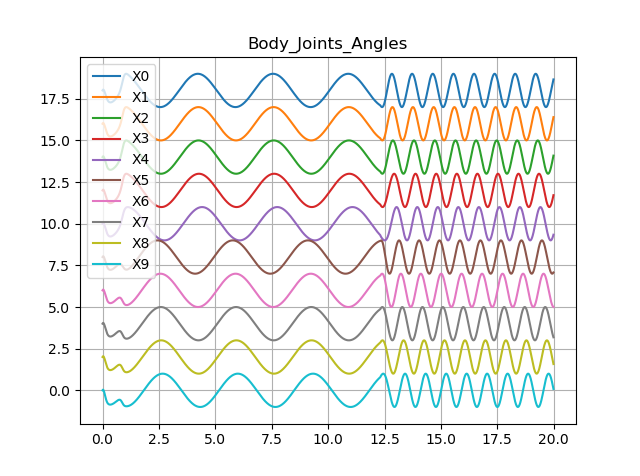
\includegraphics[width=0.9\linewidth]{figures/8g_walk_to_swim.png} 
    \caption{Joint angles for walk to swim transition} 
    \label{fig:exercise8g_results:a} 
  \end{subfigure}%% 
  \begin{subfigure}[b]{0.5\linewidth}
    \centering
    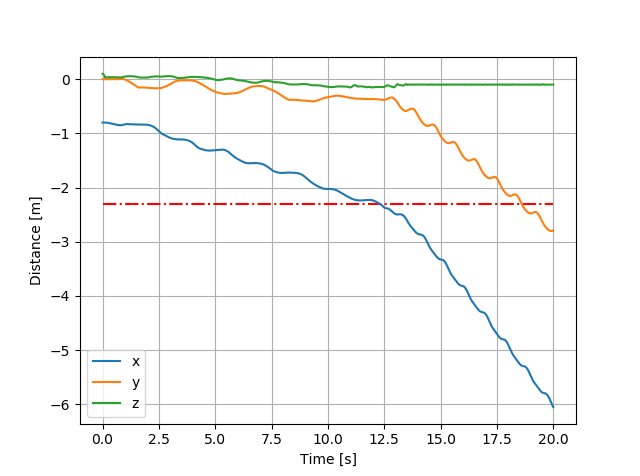
\includegraphics[width=0.9\linewidth]{figures/8g_wts_position.png} 
    \caption{Positions for walk to swim} 
    \label{fig:exercise8g_results:b} 
  \end{subfigure}
  \begin{subfigure}[b]{0.5\linewidth}
    \centering
    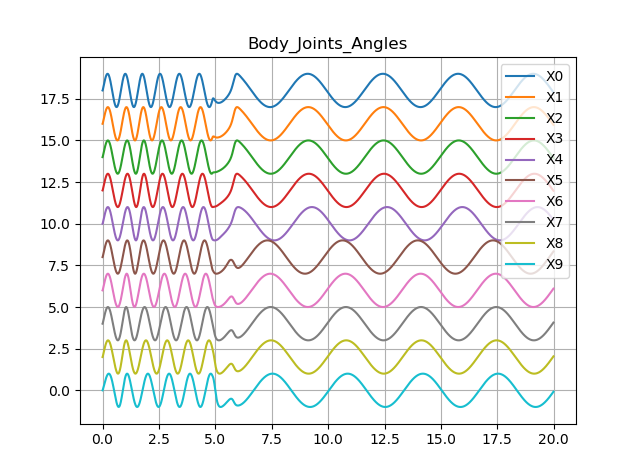
\includegraphics[width=0.9\linewidth]{figures/8g_swim_to_walk.png} 
    \caption{Joint angles for swim to walk transition} 
    \label{fig:exercise8g_results:c} 
  \end{subfigure}%% 
  \begin{subfigure}[b]{0.5\linewidth}
    \centering
    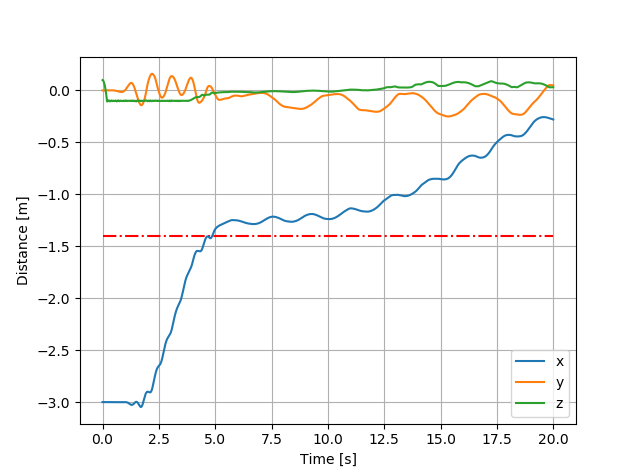
\includegraphics[width=0.9\linewidth]{figures/8g_stw_position.png} 
    \caption{Positions for walk to swim} 
    \label{fig:exercise8g_results:d} 
  \end{subfigure}
  \caption{Velocity over phase offset and oscillation amplitude}
  \label{fig:exercise8g_results} 
\end{figure}

In those graphs it shows really well the transitions, with the red dotted line showing the coordinate in x where it does the transition. After experimenting with different values, we put the transition from land to water at $-2.3[m]$ and from water to land at $-1.4[m]$. The former lets the whole body of the salamander go into the water before beginning to swim while the latter is deep into land so that the movement of the tail helps going up the slope before beginning to walk. 

In the land to water transition we can see that after the transition the salamander goes sideways because he didn't finish a whole cycle of walking before transitioning. In the water to land we can see a slight struggle for one cycle or 2, because of the slope.

The video (that can be found in \corr{\textbackslash Lab8\textbackslash Report\textbackslash simulation\_final.mp4}) shows the whole process of the lab :
\begin{enumerate}
\item Walk on land
\item Transition to water
\item Swim in water
\item Turn right (when the salamander's head position in x is over $3.5$)
\item Transition to land

\end{enumerate}

% \newpage

\bibliography{lab8}
\label{sec:references}
\bibliographystyle{ieeetr}


% \newpage

% \section*{APPENDIX}
% \label{sec:appendix}

\end{document}

%%% Local Variables:
%%% mode: latex
%%% TeX-master: t
%%% End: